\begin{figure*}[ht]
	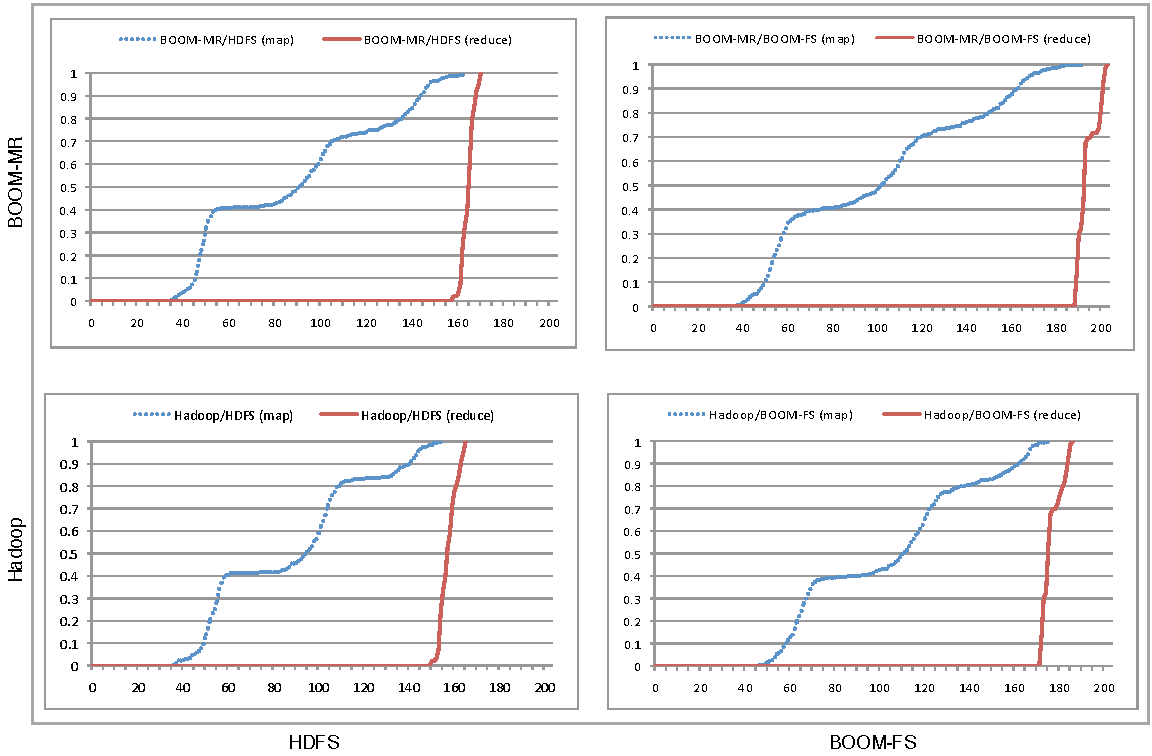
\includegraphics[width=0.95\linewidth]{graphs/fourgraphs}
% \begin{minipage}{0.5\linewidth}
%         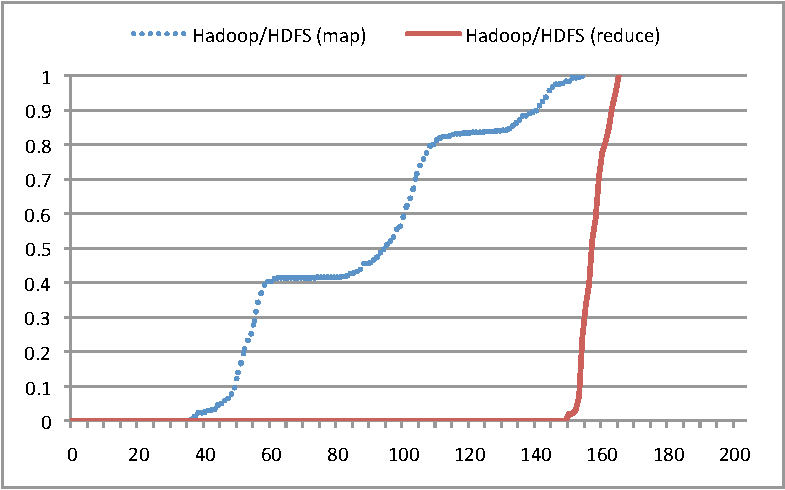
\includegraphics[width=0.95\linewidth]{graphs/hadoop_hdfs}
% \end{minipage}
% \begin{minipage}{0.5\linewidth}
%         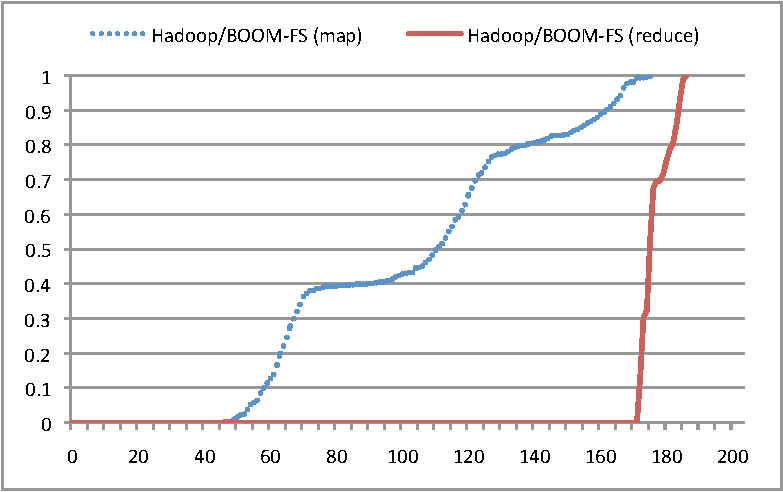
\includegraphics[width=0.95\linewidth]{graphs/hadoop_bfs}
% \end{minipage}
% \begin{minipage}{0.5\linewidth}
%         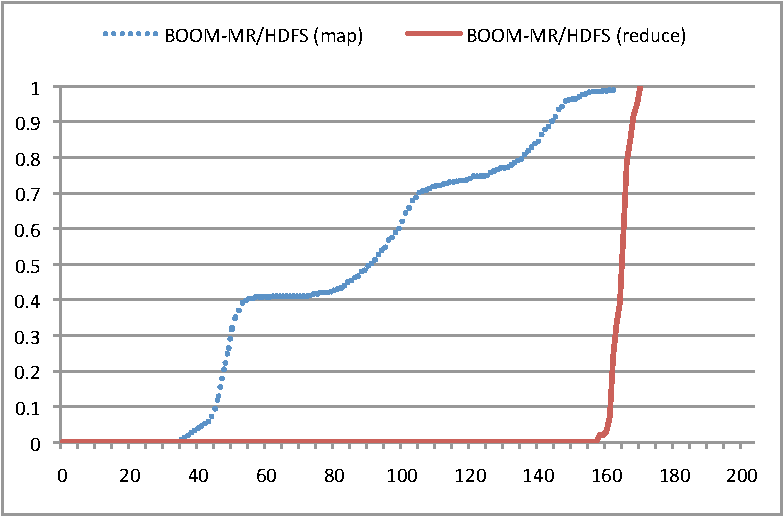
\includegraphics[width=0.95\linewidth]{graphs/bmr_hdfs}
% \end{minipage}
% \begin{minipage}{0.5\linewidth}
%         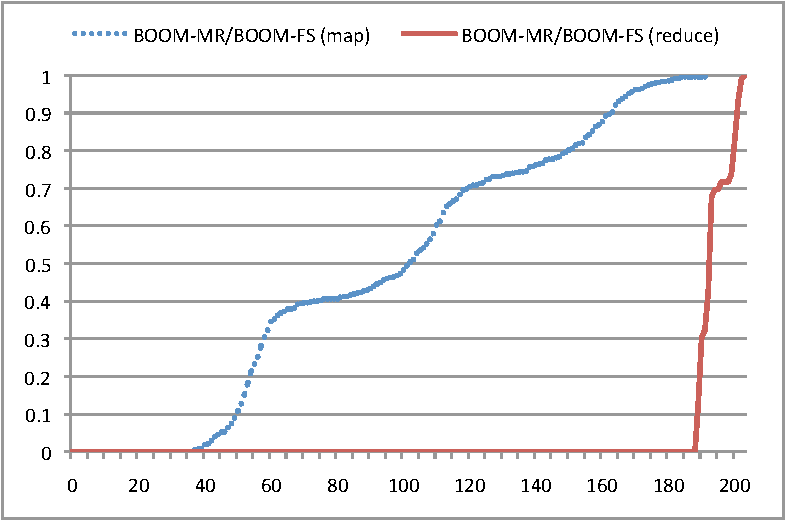
\includegraphics[width=0.95\linewidth]{graphs/bmr_bfs}
% \end{minipage}
\caption{CDFs representing the elapsed time between job startup and task
  completion for both map and reduce tasks, for all combinations of Hadoop and \BOOM-MR
  over HDFS and \BOOM-FS\@.  In each graph, the horizontal axis is
  elapsed time in seconds, and the vertical represents the percentage of tasks completed.}
\label{fig:ec2experiment}
\vspace{-8pt}
\end{figure*}

\section{Performance Validation}
\label{sec:eval}
While improved performance was not a goal of our work, we wanted to
ensure that the performance of \BOOMA was competitive with Hadoop.
We compared \BOOMA with Hadoop 18.1, using the 101-node EC2 cluster
described in Section~\ref{sec:schedeval}. The workload was a wordcount job
on a 30 GB file, using 481 map tasks and 100 reduce tasks.

Figure~\ref{fig:ec2experiment} contains four graphs comparing the performance of
different combinations of Hadoop MapReduce, HDFS, \BOOM-MR, and \BOOM-FS\@. Each
graph reports a cumulative distribution of the elapsed time in seconds from job
startup to map or reduce task completion. The map tasks complete in three
distinct ``waves.'' This is because only 2 $\times$ 100 map tasks can be
scheduled at once. Although all 100 reduce tasks can be scheduled immediately,
no reduce task can finish until all maps have been completed because each reduce
task requires the output of all map tasks.

The lower-left graph describes the performance of Hadoop running on top of HDFS,
and hence serves as a baseline for the subsequent graphs. The upper-left graph
details \BOOM-MR running over HDFS\@. This graph shows that map and reduce task
durations under \BOOM-MR are nearly identical to Hadoop 18.1. The lower-right
and upper-right graphs detail the performance of Hadoop MapReduce and \BOOM-MR
running on top of \BOOM-FS, respectively. \BOOM-FS performance is slightly
slower than HDFS, but remains competitive.

% The LATE policy presents an alternative scheme for speculative task
% execution on {\em straggler} tasks~\cite{late-sched}, in an effort to
% improve on Hadoop's policy.  There are two aspects to each policy:
% choosing which tasks to speculatively re-execute, and choosing {\TT}s
% to run those tasks.  Original Hadoop re-executes a task if its
% progress is more than 0.2 (on a scale of $[0..1]$) below the mean
% progress of similar tasks; it assigns speculative tasks using the same
% policy as it uses for initial tasks. LATE chooses tasks to re-execute
% via an {\em estimated finish time} metric based on the task's
% \emph{progress rate}. Moreover, it avoids assigning speculative tasks
% to {\TT}s that exhibit slow performance executing similar tasks, in
% hopes of preventing the creation of new stragglers.

%%The LATE policy is specified in the paper via just three lines of
%%pseudocode, which make use of three performance statistics called {\em
%%  SlowNodeThreshold}, {\em SlowTaskThreshold}, and {\em
%%  SpeculativeCap}.  The first two of these statistics correspond to
%%the 25th percentiles of progress rates across {\TT}s and across tasks,
%%respectively.  The {\em SpeculativeCap} is suggested to be set at 10\%
%%of available task slots~\cite{late-sched}.  We compute these
%%thresholds via the five Overlog rules shown in
%%Figure~\ref{fig:latePolicy}.  Integrating the rules into \BOOM-MR
%%required modifying two additional Overlog rules that identify tasks to
%%speculatively re-execute, and that choose {\TT}s for scheduling those
%%tasks.

% If a \TT asks for new a new task and there are fewer than {\em SpeculativeCap} speculative tasks running:
% \begin{enumerate}
% \item Ignore the request if the \TT progress for running tasks is below some {\em SlowNodeThreshold}
% \item Rank current running tasks by the estimated finish time
% \item Launch a copy of the highest-ranked task with progress rate below {\em SlowTaskThreshold}
% \end{enumerate}


%The primary inputs to the LATE policy are the {\em SpeculativeCap}, {\em SlowTaskThreshold} and the {\em SlowNodeThreshold} values, which provide thresholds for pruning tasks and nodes from consideration. The SpeculativeCap is a single system level query maintained in the scheduler.olg module, and is used to limit the total number of speculative map and reduce tasks. SlowTaskThreshold and SlowNodeThreshold values are categorized by the job identifier and task type (map or reduce). Selecting which tasks to speculate, and on which trackers they should execute, required changes to two queries in the first-come first-serve policy.olg module and the additional 6 queries. %shown in  Figure~\ref{fig:latePolicy}. 

%A task is only considered for speculation if its progress rate falls below the SlowTaskThreshold in its given category.  Queries L1 - L3 maintain this threshold value for each category. Query L1 determines the progress rate for a given task based on its current progress and running time. Query L2 forms a list of the progress rates for each task category. Finally, query L3 computes a SlowTaskThreshold for each task type of a job by taking the lower 25th percentile of the progress rate list. 
%The LATE policy ensures that speculative tasks execute on ``fast'' nodes by pruning \TT nodes whose rate of progress for a given task category fall below some threshold. Queries L4 - L6 maintain this threshold value for each task category. The first query L4, computes the average progress that a given \TT has made for each task category and stores that result in the taskPR table. Query L5 forms a list of the average progress rates out of each category by aggregating over the taskPR table, and the result of this query is stored in the trackerPRList table. Query L6 computes the slowNodeThreshold for each category by taking the 25th percentile of the list of rates stored in the trackerPRList table.


% \jmh{Tyson/Khaled to write one paragraph here on the size/complexity of the LATE implementation.}
% 
% \jmh{Tyson/Khaled to write on paragraph here with motivation for
% affinity scheduler here, a sketch of the policy that was
% implemented.}

% \subsection{LATE Evaluation}
% Figure~\ref{fig:ec2reduce} shows the cumulative distribution of the
% completion time for reduce task executions on EC2 under normal load,
% and with artificial extra load placed on six straggler nodes.  The
% same wordcount workload was used for this experiment but the number of
% reduce tasks was increased from $100$ to $400$ in order to produce two
% waves of reduce tasks.  The plots labeled ``No Stragglers'' represent
% normal load.  The plots labeled ``Stragglers'' and ``Stragglers
% (LATE)'' are taken under the (six node) artificial load using the
% vanilla Hadoop and LATE policies (respectively) to identify
% speculative tasks.  We do not show a CDF of the map task execution
% time since the artificial load barely affects it --- the six
% stragglers have no effect on other map tasks, they just result in a
% slower growth from just below $100\%$ to completion.
% %Figure~\ref{fig:ec2map} shows that the delay due to the loaded map stragglers only
% %affects those six nodes.  
% The first wave of $200$ reduce tasks is scheduled concurrently with
% all the map tasks. This first wave of reduce tasks will not finish
% until all map tasks have completed, which increases the completion time
% of these tasks as indicated in the right portion of the graph. The
% second wave of $200$ reduce tasks will not experience the delay due to
% unfinished map work since it is scheduled after all map tasks have
% finished. These shorter completion times are reported in the left
% portion of the graph. Furthermore, stragglers have less of an impact
% on the second wave of reduce tasks since less work (i.e., no map work)
% is being performed. Figure~\ref{fig:ec2reduce} shows this effect, and
% also demonstrates how the LATE implementation in \BOOMA handles
% stragglers much more effectively than the default speculation policy
% ported from Hadoop.  This echoes the results of Zaharia et
% al.~\cite{late-sched}
